\section*{Flujo de llamadas: User Mode vs Kernel Mode}

\begin{enumerate}
    \item \textbf{User Mode (U) - Aplicación y librerías de alto nivel}
    \begin{itemize}
        \item notepad++.exe: SetLibraryProperty (operaciones internas de la aplicación)
        \item user32.dll: CallWindowProcW, IsWindowUnicode (interacción con interfaz Windows)
        \item KernelBase.dll: WriteFile + 0x8d (función de usuario de alto nivel)
        \item ntdll.dll: ZwWriteFile (interfaz hacia la syscall)
    \end{itemize}

    \item \textbf{Kernel Mode (K) - Operaciones de bajo nivel y hardware}
    \begin{itemize}
        \item FLTMGR.SYS: FltPerformSynchronousIo, FltSetCancelCompletion (filtro de sistema de archivos)
        \item ntoskrnl.exe: IoCallDriver, NtDeviceIoControlFile, NtWriteFile (operaciones sobre drivers y disco)
    \end{itemize}
\end{enumerate}

\noindent
\textbf{Interpretación:} El flujo comienza en User Mode con la aplicación y librerías de alto nivel, y termina en Kernel Mode ejecutando operaciones de escritura en disco con privilegios elevados.

\begin{center}
    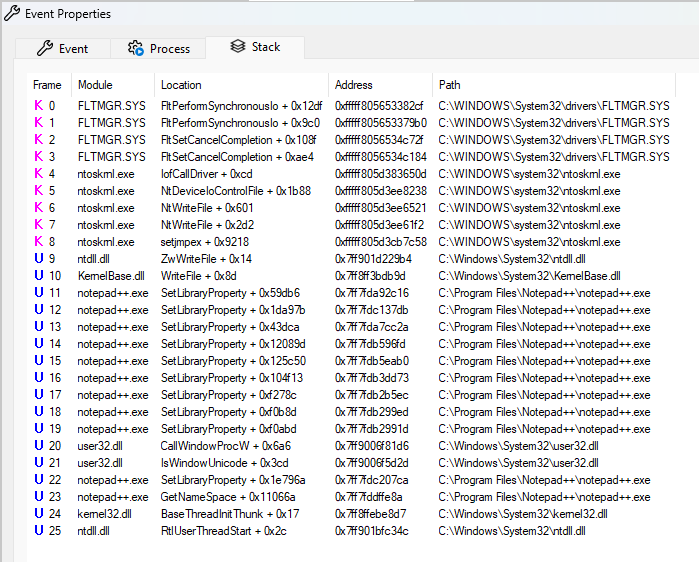
\includegraphics[width=0.95\textwidth]{figures/fig-syscall-path.png}
\end{center}